% Created 2022-07-25 Mon 16:54
% Intended LaTeX compiler: pdflatex
\documentclass[presentation,aspectratio=1610]{beamer}
\usepackage[utf8]{inputenc}
\usepackage[T1]{fontenc}
\usepackage{graphicx}
\usepackage{grffile}
\usepackage{longtable}
\usepackage{wrapfig}
\usepackage{rotating}
\usepackage[normalem]{ulem}
\usepackage{amsmath}
\usepackage{textcomp}
\usepackage{amssymb}
\usepackage{capt-of}
\usepackage{hyperref}
\usepackage{khpreamble, euscript}
\DeclareMathOperator{\atantwo}{atan2}
\newcommand*{\ctrb}{\EuScript{C}}
\newcommand*{\obsv}{\EuScript{O}}
\usetheme{default}
\author{Kjartan Halvorsen}
\date{\today}
\title{State feedback}
\hypersetup{
 pdfauthor={Kjartan Halvorsen},
 pdftitle={State feedback},
 pdfkeywords={},
 pdfsubject={},
 pdfcreator={Emacs 26.3 (Org mode 9.4.6)}, 
 pdflang={English}}
\begin{document}

\maketitle

\section{Apollo moon lander}
\label{sec:orga06b02f}
\begin{frame}[label={sec:orgf6d7efd}]{Example - The Apollo lunar module}
\begin{center}
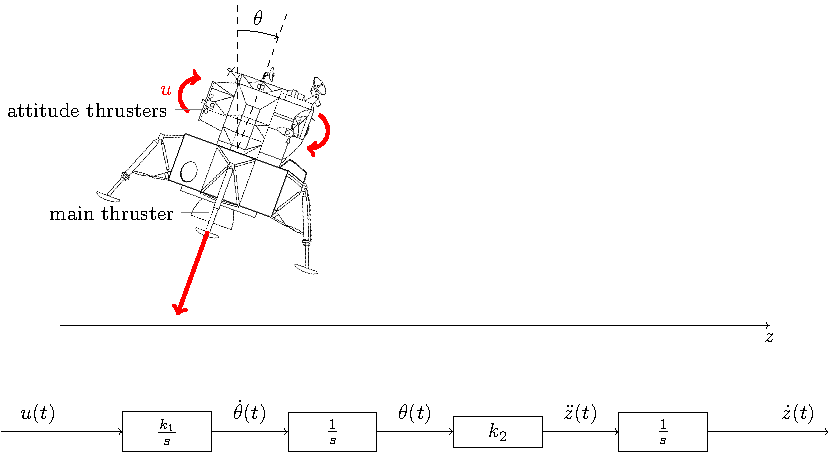
\includegraphics[width=\linewidth]{fig-apollo}
\end{center}
\end{frame}

\begin{frame}[label={sec:orgdb09905}]{Example - The Apollo lunar module}
State variables: \(x = \begin{bmatrix} x_1 & x_2 & x_3 \end{bmatrix}^T = \begin{bmatrix} \dot{\theta} & \theta & \dot{z} \end{bmatrix}^T\). With dynamics
\[ \begin{cases} \dot{x}_1 =  \ddot{\theta} = k_1 u\\ \dot{x}_2 = \dot{\theta} = x_1\\ \dot{x}_3 = \ddot{z} = k_2\theta = k_2x_2 \end{cases} \]

\[ \dot{x} = \begin{bmatrix} \dot{x}_1\\\dot{x}_2\\\dot{x}_3\end{bmatrix} = \underbrace{\begin{bmatrix} \textcolor{red!60!black}{0} & \textcolor{red!60!black}{0} &\textcolor{red!60!black}{0} \\\textcolor{red!60!black}{1} & \textcolor{red!60!black}{0}& \textcolor{red!60!black}{0}\\ \textcolor{red!60!black}{0}& \textcolor{red!60!black}{k_2} &\textcolor{red!60!black}{0} \end{bmatrix}}_{A} \begin{bmatrix} x_1\\x_2\\x_3\end{bmatrix} + \underbrace{\begin{bmatrix} \textcolor{red!60!black}{k_1} \\ \textcolor{red!60!black}{0} \\\textcolor{red!60!black}{0}  \end{bmatrix}}_{B} u \]
\end{frame}


\begin{frame}[label={sec:orgd1e9a7e}]{Example - The Apollo lunar module}
 \begin{align*}
  x(kh+h) &= \mathrm{e}^{Ah} x(kh) + \int_{0}^{h} \mathrm{e}^{As} B u(kh+h-s) ds\\
   &= \underbrace{\mathrm{e}^{Ah}}_{\Phi(h)} x(kh) + \underbrace{\left(\int_{0}^h \mathrm{e}^{As} B ds \right)}_{\Gamma(h)} u(kh)\\
   &= \begin{bmatrix} 1 & 0 & 0\\h & 1 & 0\\\frac{h^2k_2}{2} & hk_2 & 1\end{bmatrix} x(kh) + k_1 \begin{bmatrix} h\\ \frac{h^2}{2} \\ \frac{k_2 h^3}{6} \end{bmatrix} u(kh)
\end{align*}
\end{frame}

\section{Stability}
\label{sec:orgcffc210}
\begin{frame}[label={sec:org8069c25}]{Stability}
\end{frame}
\begin{frame}[label={sec:org3f34a4d}]{Eigenvalues and eigenvectors}
\alert{Definition} The eigenvalues \(\lambda_i  \in \mathbb{R}\) and eigenvectors \(v_i \in \mathbb{R}^n\) of a matrix \(\Phi \in \mathbb{R}^{n\times{}n}\) are the \(n\) pairs \((\lambda_i, v_i \neq 0 ), \; i=1,2,\ldots,n\) that satisfy
\[ \Phi v_i = \lambda_i v_i \]
\end{frame}

\begin{frame}[label={sec:orga63cfd2}]{Stability}
The system
\begin{equation*}
x(k+1)=\Phi x(k), \ \ x(0)=x_0
\end{equation*}
is \alert{stable} if  \(\underset{t\to\infty}{\lim}x(kh)=0, \quad \forall\;  x_0\in\Bbb{R}^n\).

A necessary and sufficient requirement for stability is that \alert{all the eigenvalues of \(\Phi\) are inside the unit circle.}

The \alert{eigenvalues} of \(\Phi\) are the  \alert{poles} of the system.
\end{frame}

\begin{frame}[label={sec:org38dc8b1}]{Eigenvalues and eigenvectors - exercise}
\alert{Activity} Verify that the vector
\[ v = \begin{bmatrix}1\\0\end{bmatrix}\]
is an eigenvector of
\[ \Phi = \begin{bmatrix} 2 & 0\\0 & \frac{1}{2} \end{bmatrix}. \]
What is the corresponding eigenvalue?
\end{frame}

\section{Controllability and observability}
\label{sec:org41f8fd3}

\begin{frame}[label={sec:orgf8a8662}]{Controllability}
Controllability is the answer to the question \emph{Can we drive the state of the system to any location in the state space by a suitable input sequence \(u(k),\; k=0,1,2,\ldots,n-1\)?}

Consider
\[ x(k+1) = \Phi x(k) + \Gamma u(k), \quad x(0)= x_0 \]
with solution
\begin{equation}
\begin{split}
x(n) &= \Phi^nx(0) + \Phi^{n-1}\Gamma u(0) + \Phi^{n-2}\Gamma u(1) + \cdots + \Gamma u(n-1)\\
     &= \Phi^nx(0) + W_c U, 
\end{split}
\end{equation}
where
\begin{align*}
W_c &= \bbm \Gamma & \Phi\Gamma & \cdots & \Phi^{n-1}\Gamma\ebm\\
U &= \bbm u(n-1) & u(n-2) & \cdots & u(0) \ebm\transp
\end{align*}
\end{frame}

\begin{frame}[label={sec:org020d0e3}]{Controllability}
To find the input sequence \(u(k)\) that takes the state from  \(x(0)=x_0\) to \(x(n) = x_d\) we may solve for \(U\) in the equation
\[ x_d = \Phi^nx_0 + W_cU.\]

\[ U = W_c\inv \left(x_d - \Phi^nx(0)\right) \]

This is possible when the matrix \(W_c\) is \alert{invertible}:

The state-space system above is controllable if and only if the \emph{Controllability matrix} \(W_c\)  has rank \(n\), i.e. 
\[ \det W_c \neq 0.\]
\end{frame}

\section{Observability}
\label{sec:org2a5a093}
\begin{frame}[label={sec:orgf54431d}]{Observability}
\footnotesize

Observability is the answer to the question "Can we determine the initial state \(x(0)\) from measurements \(y(k), \; k=0,1,2,\ldots, n-1\)?"

The first \(n\) values of the output sequence (with \(u=0\))are given by
\begin{align*}
y(0) &= Cx(0)\\
y(1) &= Cx(1) = C \Phi x(0)\\
& \vdots\\
y(n-1) &= Cx(n-1) = C\Phi^{n-1} x(0).
\end{align*}
This gives the equation
\[ \bbm C\\C\Phi\\\vdots\\C\Phi^{n-1} \ebm x(0) = \bbm y(0)\\y(1))\\\vdots\\ y(n-1)\ebm \]

\pause
\alert{Activity} Solve for \(x(0)\)!

\pause

\[ \text{possible iff} \quad \[W_o = \bbm C\\C\Phi\\\vdots\\C\Phi^{n-1} \ebm\quad \text{has full rank.}\]
\end{frame}

\begin{frame}[label={sec:org47617e6}]{Observability, contd}
The equation
\[ \bbm C\\C\Phi\\\vdots\\C\Phi^{n-1} \ebm x(0) = \bbm y(0)\\y(1) - C\Gamma u(0)\\\vdots\\ y(n-1) - CW_c U\ebm \]
 can be solved for \(x(0)\) if and only if the matrix 
\[W_o = \bbm C\\C\Phi\\\vdots\\C\Phi^{n-1} \ebm\] has full rank. If this is the case, the system is said to be \alert{observable}.
\end{frame}

\section{State feedback}
\label{sec:orgb507b0f}
\begin{frame}[label={sec:org4db06e7}]{State feedback control}
\end{frame}
\begin{frame}[label={sec:org28aefd5}]{State feedback control}
Given
 \begin{equation}
 \begin{split}
  x(k+1) &= \Phi x(k) + \Gamma u(k)\\
  y(k) &= C x(k)
 \end{split}
 \label{eq:ssmodel}
\end{equation}
and measurements (or an estimate) of the state vector \(x(k)\). 

\alert{Linear state feedback} is the control law
\begin{equation*}
\begin{split}
 u(k) &= f\big((x(k), u_c(k)\big) = -l_1x_1(k) - l_2x_2(k) - \cdots - l_n x_n(k) + l_0u_c(k)\\
      &= -Lx(k) + l_0u_c(k), 
\end{split}
\end{equation*}
where \[ L = \bbm l_1 & l_2 & \cdots & l_n \ebm. \]
\pause
\alert{Activity} Substitute the control law  \(u = l_0u_c(k) - Lx(k)\) into the state-space model \eqref{eq:ssmodel}
\pause

 \begin{equation}
 \begin{split}
  x(k+1) &= \left(\Phi -\Gamma L \right) x(k) + l_0\Gamma u_c(k)\\
  y(k) &= C x(k)
 \end{split}
 \label{eq:closedloop}
\end{equation}
\end{frame}

\begin{frame}[label={sec:org13ecd38}]{Pole placement by state feedback}
Given a desired placement of the closed-loop poles \(p_1, p_2, \ldots, p_n\), being roots of the desired characteristic polynomial
\begin{equation}
a_c(z) = (z-p_1)(z-p_2)\cdots(z-p_n) = z^n + \alpha_1 z^{n-1} + \cdots \alpha_n.
\label{eq:desiredpoles}
\end{equation}

\pause
Linear state feedback gives the system
 \begin{equation}
 \begin{split}
  x(k+1) &= \left(\Phi -\Gamma L \right) x(k) + l_0\Gamma u_c(k)\\
  y(k) &= C x(k)
 \end{split}
 \label{eq:closedloop}
\end{equation}
with characteristic polynomial
\begin{equation}
\det\left(zI - (\Phi - \Gamma L)\right) = z^n + \beta_1(l_1,\ldots,l_n) z^{n-1} + \cdots \beta_n(l_1, \ldots, l_n).
\label{eq:poles}
\end{equation}

\pause
Set the coefficients of the desired characteristic polynomial \eqref{eq:desiredpoles} equal to the coefficients of \eqref{eq:poles} to obtain the system of equations
\begin{equation*}
\begin{split}
\beta_1(l_1, \ldots, l_n) &= \alpha_1\\
\beta_2(l_1, \ldots, l_n) &= \alpha_2\\
&\vdots\\
\beta_n(l_1, \ldots, l_n) &= \alpha_n
\end{split}
\label{eq:coeffs}
\end{equation*}
\end{frame}

\begin{frame}[label={sec:org88d3142}]{Pole placement by state feedback}
The system of equations
\begin{equation*}
\begin{split}
\beta_1(l_1, \ldots, l_n) &= \alpha_1\\
\beta_2(l_1, \ldots, l_n) &= \alpha_2\\
&\vdots\\
\beta_n(l_1, \ldots, l_n) &= \alpha_n
\end{split}
\label{eq:coeffs}
\end{equation*}
is always linear in the parameters of the controller, henc
\begin{equation*}
M L\transp = \alpha,
\end{equation*}
where \(\alpha\transp = \bbm \alpha_1 & \alpha_2 & \cdots & \alpha_n \ebm.\)
\end{frame}

\begin{frame}[label={sec:org606750d}]{Pole placement and controllability}
It can be shown that the controllability matrix
\[W_c = \bbm \Gamma & \Phi\Gamma & \cdots & \Phi^{n-1}\Gamma\ebm\]
is a factor of the matrix \(M\)
\[ M = \bar{M} W_c. \] Hence, in general, the equations
\begin{equation}
\bar{M}W_c L\transp = \alpha \qquad \Rightarrow \qquad L\transp = W_c^{-1}\bar{M}^{-1}\alpha
\label{eq:poleplace}
\end{equation}
only has a solution if \(W_c\) is invertible, that is when the system is \emph{controllable}.

 Note that the equations \eqref{eq:poleplace} may also have solutions when the system is not controllable, if  \alert{\(\alpha\) is in the column space of \(M\)}. That is 
\[ \alpha = b_1 M_{:,1} + b_2M_{:,2} + \cdots + b_M_{:,m}, \; m < n \]
\end{frame}

\begin{frame}[label={sec:orgd466022},fragile]{Pole placement by state feedback}
 Given a desired placement of the closed-loop poles \(p_1, p_2, \ldots, p_n\), being roots of the desired characteristic polynomial
\begin{equation}
a_c(z) = (z-p_1)(z-p_2)\cdots(z-p_n) = z^n + \alpha_1 z^{n-1} + \cdots \alpha_n.
\label{eq:desiredpoles}
\end{equation}
and closed-loop system
 \begin{equation}
 \begin{split}
  x(k+1) &= \left(\Phi -\Gamma L \right) x(k) + l_0\Gamma u_c(k)\\
  y(k) &= C x(k)
 \end{split}
 \label{eq:closedloop}
\end{equation}

The Matlab (\emph{control systems toolbox}) has methods for computing the gain vector \(L\)

\begin{enumerate}
\item \alert{Ackerman's method} 
\begin{verbatim}
L = acker(Phi, Gamma, pd)
\end{verbatim}
\item \alert{Numerically more stable method} 
\begin{verbatim}
L = place(Phi, Gamma, pd)
\end{verbatim}
\end{enumerate}
\end{frame}

\begin{frame}[label={sec:orgd8f4570}]{The reference input gain \(l_0\)}
The closed-loop state space system
\begin{equation*}
\begin{split}
 x(k+1) &= \underbrace{\left(\Phi -\Gamma L \right)}_{\Phi_c} x(k) + l_0\Gamma u_c(k)\\
 y(k) &= C x(k)
\end{split}
\end{equation*}
has the steady-state solution (\(x(k+1)=x(k)\)) for constant reference signal \(u_c(k) = u_{c,f}\)
\[ y_f = l_0 C(I - \Phi_c)^{-1}\Gamma u_{c,f}.\]
We want \(y_f =  u_{c,f}\),
\[ \Rightarrow \qquad l_0 = \frac{1}{C(I-\Phi_c)^{-1}\Gamma}\]
\end{frame}

\section{Exercise}
\label{sec:org5a40279}

\begin{frame}[label={sec:orga7a2e33}]{Exercise - The harddisk drive arm}
\footnotesize
The model of the arm of the harddisk drive
\begin{center}
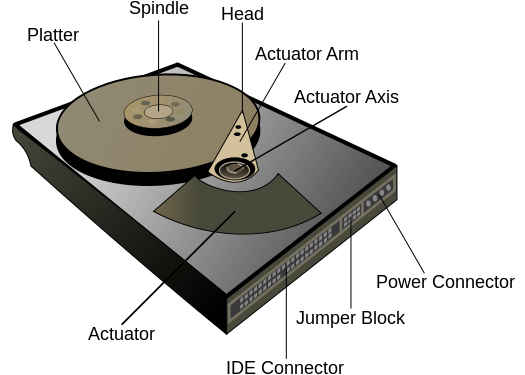
\includegraphics[width=0.2\linewidth]{../../figures/hard-drive.png}
\end{center}
can, with suitable choice of sampling period, be written

\[x(k+1) = \Phi x(k) + \Gamma u(k) = \begin{bmatrix} 1 & 0.4\\ 0 &1 \end{bmatrix} x + \begin{bmatrix}0.16\\0.8\end{bmatrix}u.\]
With linear state feedback \(u(k) = -Lx(k) + l_0u_c(k)\) the closed-loop system is
\begin{equation*}
   \begin{split}
    x(k+1) &= \left(\Phi -\Gamma L \right) x(k) + l_0\Gamma u_c(k)\\
           &= \begin{bmatrix} 1-0.16l_1 & 0.4 - 0.16l_2\\-0.8l_1 & 1-0.8l_2\end{bmatrix} x(k) + l_0\Gamma u_c(k).
   \end{split}
\end{equation*}

\alert{Determine} the characteristic polynomial of the closed-loop system \(\det \Big( zI - (\Phi - \Gamma L)\Big)\)
\end{frame}
\end{document}